% 1977 年河南卷第七题：长方体 ABCD-A1B1C1D1（顶面 A1B1C1D1），
% 体对角线 A1C（虚线）与底面所成角 α 标在 C 处，底面对角线 AC、BD 夹角 β 标在中心（按源卷第 3 页布局）
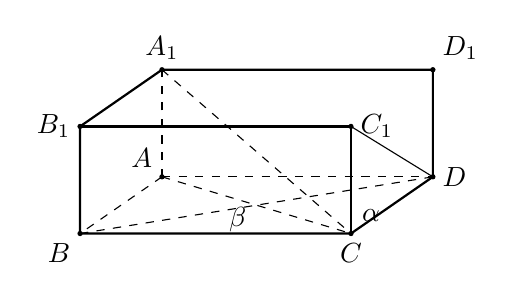
\begin{tikzpicture}[scale=0.8]
  \coordinate (B) at (0,0.8);
  \coordinate (C) at (4.3,0.8);
  \coordinate (D) at (5.6,1.7);
  \coordinate (A) at (1.3,1.7);
  \coordinate (B1) at (0,2.5);
  \coordinate (C1) at (4.3,2.5);
  \coordinate (D1) at (5.6,3.4);
  \coordinate (A1) at (1.3,3.4);
  \draw[thick] (B)--(C)--(D)--(D1)--(A1)--(B1)--cycle;
  \draw[thick] (B)--(B1);
  \draw[thick] (C)--(C1);
  \draw[thick] (A1)--(D1);
  \draw[thick] (B1)--(C1);
  \draw[thin] (C1)--(D);
  \draw[dashed] (A)--(B);
  \draw[dashed] (A)--(D);
  \draw[dashed] (A)--(A1);
  \draw[dashed] (A)--(C);
  \draw[dashed] (B)--(D);
  \draw[dashed] (A1)--(C);
  \fill (A) circle (1.2pt) node[above left] {$A$};
  \fill (B) circle (1.2pt) node[below left] {$B$};
  \fill (C) circle (1.2pt) node[below] {$C$};
  \fill (D) circle (1.2pt) node[right] {$D$};
  \fill (A1) circle (1.2pt) node[above] {$A_1$};
  \fill (B1) circle (1.2pt) node[left] {$B_1$};
  \fill (C1) circle (1.2pt) node[right] {$C_1$};
  \fill (D1) circle (1.2pt) node[above right] {$D_1$};
  \node at (4.62,1.08) {$\alpha$};
  \node at (2.5,1.02) {$\beta$};
\end{tikzpicture}
